\documentclass[TeamE-eindrapport]{subfiles}

\begin{document}
	
	\chapter{Classificatie}
	
	\section{Wat is classificatie}
	
	Classificatie is een machine learning techniek die binnen het gebied van supervised learning valt. Bij deze methode worden gegevens in een dataset ingedeeld in verschillende klassen, het kan worden uitgevoerd op zowel gestructureerde als ongestructureerde gegevens. Het proces begint met het voorspellen van de klasse van bepaalde datapunten.. De klassen worden vaak aangeduid als target, label of categorie. Het ultieme doel van classificatie is om te bepalen in welke categorie de nieuwe gegevens zullen vallen.
	
	Om het concept een beetje beter te kunnen begrijpen bekijken we een eenvoudige voorstelling van de toepassing in verband met tumoren. Hierbij willen we aan de hand van classificatie onderzoeken of een tumor goedaardig of kwaadaardig is. Dit is een voorbeeld van een binaire classificatie aangezien er slechts twee klassen kunnen zijn, namelijk goedaardig of kwaadaardig.
	
	
	\section{Terminologie}
	
	De \textbf{classifier} is een algoritme dat gebruikt wordt om de invoergegevens toe te wijzen aan een specifieke categorie. In ons geval heeft de classifier trainingsgegevens nodig om te begrijpen wat het verband is tussen de gegeven invoervariabelen en de klasse. Als de classifier nauwkeurig getraind is, kan deze worden gebruikt om na te gaan of de tumor goedaardig of kwaadaardig is.
	
	Het \textbf{classificatiemodel} voorspelt de klasse of categorie van de gegevens aan de hand van de invoergegevens die tijdens de training zijn verstrekt.
	
	Het \textbf{feature} of kenmerk is een meetbare eigenschap van iets dat je waarneemt. Bij tumorclassificatie kunnen bijvoorbeeld grootte, vorm, compositie en locatie van het beeld dienen als kenmerken.
	
	Er bestaan ook classificaties met \textbf{meerdere klassen} of \textbf{meerdere labels}. Bij meerdere klassen wordt elk voorbeeld toegewezen aan één label, zoals bijvoorbeeld het identificeren van verschillende soorten dieren.  Bij meerdere labels wordt elk voorbeeld toegewezen aan een reeks labels, zo kan een afbeelding meerdere objecten bevatten.
	
	\textbf{Overfitting} treedt op wanneer een model te specifiek is voor de trainingsgegevens en slecht presteert op nieuwe, ongeziene gegevens. \textbf{Onderfitting} daarentegen treedt op wanneer het model te eenvoudig is en niet in staat is de complexiteit van de gegevens vast te leggen.
	
	
	\section{Enkele toepassingen}
	\begin{itemize}
		\item \textbf{Beeldherkenning:} Classificatie wordt vaak gebruikt in beeldherkenningstoepassingen, zoals het identificeren van objecten in foto's of video's.
		
		\item \textbf{Tekstclassificatie:} Hier wordt classificatie gebruikt om tekst te categoriseren, bijvoorbeeld het identificeren van spam-e-mails of het toewijzen van artikelen aan specifieke onderwerpen.
		
		\item \textbf{Medische diagnose:} Naast het eerder genoemde voorbeeld van tumorklassificatie, wordt classificatie ook toegepast op het diagnosticeren van verschillende medische aandoeningen op basis van verzamelde gegevens.
		
	\end{itemize}
	
	
	\begin{figure}
		\centering
		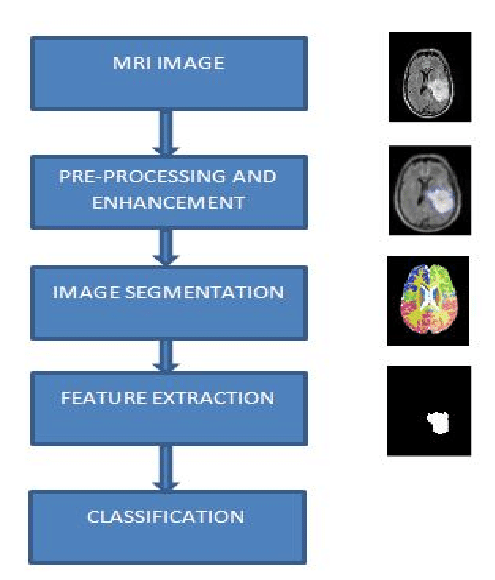
\includegraphics[width=.5\textwidth]{tumor}
		\caption{Classificatie van een tumor. De eerste stap is de voorbewerking en verbetering van de MRI afbeelding. Fijnere details worden verbeterd en de ruis wordt uit het beeld gehaald. Bij image segmentation wordt het beeld opgedeeld in verschillende delen of segmenten om het beter te kunnen analyseren. Voor de features wordt rekening gehouden met bepaalde parameters, zoals grootte, vorm, compositie en locatie van het beeld. Volgens de resultaten die zijn verkregen uit de feature-extractie, wordt de classificatie van de tumor uitgevoerd.}
	\end{figure}
	
\end{document}